\documentclass[output=paper,colorlinks,citecolor=brown]{langscibook}
\ChapterDOI{10.5281/zenodo.12090432}
\author{Felix Kpogo\affiliation{Boston University} and Alexandra Kohut\affiliation{Boston University}\orcid{} and Charles B. Chang\affiliation{Boston University}\orcid{0000-0002-3537-2053}}
\title{Expressing diminutive meaning in heritage Twi: The role of complexity and language-specific preferences}
\abstract{Twi (Akan) and English can both express diminutive meaning using a morphological strategy (diminutive suffix) or a syntactic strategy (adjectival construction), but they differ with respect to native-speaker preferences -- morphological in Twi, syntactic in English. Each strategy in Twi, moreover, is associated with different types of complexity (morphological, phonological, lexical, discourse-pragmatic, and/or inhibitory). In this study, we examined whether English-dominant, second-generation (G2) speakers of Twi in the US would express diminutive meaning in Twi differently from first-generation (G1) speakers. Results from elicited production suggest that G2 does indeed differ from G1 in this respect: whereas G1 relies on the morphological strategy, G2 relies on the syntactic strategy, producing adjectives post-nominally in accordance with Twi syntax. These results are discussed in light of variation in G2 speakers' morphological awareness and verbal fluency in Twi. Overall, our findings suggest that both the incremental complexity of linguistic options within a bilingual language repertoire and cross-linguistic influence at the level of preferences play a role in explaining G2's diminutive production.}
  


\IfFileExists{../localcommands.tex}{%hack to check whether this is being compiled as part of a collection or standalone
   \usepackage{tabularx,multicol}
\usepackage{url}
\urlstyle{same}
\usepackage{multirow}

\usepackage{stmaryrd}
\usepackage{soul}
\usepackage{enumitem}

\usepackage{siunitx}
\sisetup{group-digits=none}

\usepackage{langsci-optional}
\usepackage{langsci-lgr}
\usepackage{langsci-textipa}
\usepackage{langsci-branding}

\usepackage{tikz-qtree}

\usepackage{pgfplots}
\usepackage{qtree}
\qtreecenterfalse
\usepackage{tree-dvips}
\usepackage{subcaption}

\let\clipbox\undefined
\usepackage{adjustbox}
\usepackage[linguistics, edges]{forest}
\usepackage{langsci-gb4e}

% ORCIDs in langsci-affiliations 
\usepackage{orcidlink}
\SetupAffiliations{orcid placement=before}
\definecolor{orcidlogocol}{cmyk}{0,0,0,1}
\RenewDocumentCommand{\LinkToORCIDinAffiliations}{ +m }
  {%
    \orcidlink{#1}\,%
  }

   \newcommand*{\orcid}[1]{}


\makeatletter
\let\thetitle\@title
\let\theauthor\@author
\makeatother

\newcommand{\togglepaper}[1][0]{
   \bibliography{../localbibliography}
   \papernote{\scriptsize\normalfont
     \theauthor.
     \titleTemp.
     To appear in:
     E. Di Tor \& Herr Rausgeberin (ed.).
     Booktitle in localcommands.tex.
     Berlin: Language Science Press. [preliminary page numbering]
   }
   \pagenumbering{roman}
   \setcounter{chapter}{#1}
   \addtocounter{chapter}{-1}
}

\newbool{bookcompile}
\booltrue{bookcompile}
\newcommand{\bookorchapter}[2]{\ifbool{bookcompile}{#1}{#2}}


\forestset{
  my nice empty nodes/.style={% modified from manual page 52
    for tree={
      calign=fixed edge angles,
      calign angle=50,
    },
    delay={
      where n children=0{
        if content={}{
          content=\strut,
          anchor=north,
        }{
          align=center
        },
      }{
        if content={}{
          shape=coordinate,
          for parent={
            for children={
              anchor=north
            }
          }
        }{}
      }
    },
  },
  my pretty nice empty nodes/.style={
    for tree={
      calign=fixed edge angles,
      calign angle=50,
      parent anchor=south,
      delay={
        where n children=0{
          if content={}{
            content=\strut,
            anchor=north,
          }{
            align=center
          },
        }{
          if content={}{
            inner sep=0pt,
            edge path={\noexpand\path [\forestoption{edge}] (!u.parent anchor) -- (.south)\forestoption{edge label};}
          }{}
        }
      }
    }
  }
}


\newcommand{\sem}[1]{\mbox{$[\![$#1$]\!]$}}
\newcommand{\type}[1]{\ensuremath{\left \langle #1 \right \rangle }}
\newcommand{\lam}{\ensuremath{\lambda}}
\renewcommand{\and}{$\wedge$ }
\newcommand{\bex}{\begin{exe}}
\newcommand{\eex}{\end{exe}}
\newcommand{\bit}{\begin{itemize}}
\newcommand{\eit}{\end{itemize}}
\newcommand{\ben}{\begin{enumerate}}
\newcommand{\een}{\end{enumerate}}

\newcommand{\gcs}[1]{\textcolor{blue}{[gcs: #1]}}
\newcommand{\ash}[1]{\textcolor{orange}{[ash: #1]}}
\newcommand{\ngn}[1]{\textcolor{purple}{[ngn: #1]}}

\newcommand{\firstrefdash}{}


\forestset{
fairly nice empty nodes/.style={
delay={where content={}
{shape=coordinate, for siblings={anchor=north}}{}},
for tree={s sep=4mm}
}
}



   %% hyphenation points for line breaks
%% Normally, automatic hyphenation in LaTeX is very good
%% If a word is mis-hyphenated, add it to this file
%%
%% add information to TeX file before \begin{document} with:
%% %% hyphenation points for line breaks
%% Normally, automatic hyphenation in LaTeX is very good
%% If a word is mis-hyphenated, add it to this file
%%
%% add information to TeX file before \begin{document} with:
%% %% hyphenation points for line breaks
%% Normally, automatic hyphenation in LaTeX is very good
%% If a word is mis-hyphenated, add it to this file
%%
%% add information to TeX file before \begin{document} with:
%% \include{localhyphenation}
\hyphenation{
    par-a-digm
    peri-phras-tic
    mor-pho-pho-nol-o-gy
}

\hyphenation{
    par-a-digm
    peri-phras-tic
    mor-pho-pho-nol-o-gy
}

\hyphenation{
    par-a-digm
    peri-phras-tic
    mor-pho-pho-nol-o-gy
}

    \bibliography{localbibliography}
    \togglepaper[23]
}{}


\shorttitlerunninghead{Expressing diminutive meaning in heritage Twi}
\begin{document}
\SetupAffiliations{mark style=none}
\shorttitlerunninghead{Expressing diminutive meaning in heritage Twi}
\maketitle

\section{Introduction}
\label{IntroSec}

When presented with variable input, heritage speakers (HSs) tend to simplify complex forms in the heritage language \citep[HL; see][]{KimJH2007, IsurinIvanovaSullivan2008, IvanovaSullivan2014, ScontrasFuchsPolinsky2015, ScontrasPolinskyTsaiMai2017}, resulting in systematic differences between their grammars and those of native speakers who continue to be dominant in the language.\footnote{Following research arguing that HSs should be considered part of a continuum of native speakers \citep{RothmanTreffersDaller2014, WieseAlexiadouAllenBunkGagarinaIefremenkoMartynovaPashkovaRizouSchroederShadrovaSzucsichTracyTsehayeZerbianZuban2022}, we use the term ``heritage speaker'' not in opposition with ``native speaker'', but rather in the sense of ``switched-dominance bilingual''~-- that is, in contrast to the acquisition profile often assumed for native speakers who continue to be dominant in the target language (i.e., a profile that involves early, continuous, and socially robust exposure, but that may or may not be monolingual).} Such differences, often observed in ``interface'' phenomena, have been attributed to the greater vulnerability of structures governed by an interface (e.g., the syntax-pragmatics interface) as compared with those situated within core domains of the grammar, which tend to be more resistant to simplification and reanalysis by HSs \citep{HulkMuller2000, Sorace2000, TsimpliSoraceHeycockFiliaci2004}. 

In the current study, we examined the use of diminutives in the Twi of English-dominant HSs as a means of further investigating HSs' tendency towards simplification in the context of multiple linguistic options with different kinds of complexity.\footnote{The term ``Twi'' is used in this paper as a cover term to refer primarily to the Asante and Akuapem dialects of Akan. The term ``Akan'' is a generic name for at least eleven dialects, among which Fante, Asante, and Akuapem have achieved literary status. Asante and Akuapem, plus some other dialects, are often referred to collectively as Twi.} The linguistic options of interest here are two strategies for expressing the notion of ``smallness'' in Twi: (1) a diminutive morpheme \textit{-ba}/\textit{-wa} (e.g., \textit{sekan-ba} `machete-\textsc{dim}' $\rightarrow$ \textit{sekamma} `knife') and (2) an adjectival construction using the word \textit{ketewa} `little' (e.g., \textit{sekan ketewa} `knife', lit. `machete little'). Crucially, these options are associated with different complexities for an English-dominant HS. On the one hand, the diminutive morpheme is complex in terms of transparency, allomorphy, and productivity (see \sectref{DimExpSec}). On the other hand, the adjectival construction is complex in terms of morphosyntactic conflict with English, given that adjectives are generally post-nominal in Twi but pre-nominal in English.

Because both of the above options for expressing diminutive meaning exist in the HL (Twi) and the majority language (English), our focus in this study was not on cross-linguistic differences in grammaticality, but rather on cross-linguistic differences in \textsc{preferences} for one option vs. the other. In particular, we examined whether second-generation (G2) Twi speakers in the US, under the influence of different linguistic preferences for English, would exhibit linguistic preferences for Twi that diverged from those of first-generation (G1) Twi speakers in the same environment. Under the assumption that they would, we also examined whether individual differences among G2 speakers in the strength of their observed preferences would be related to aspects of their HL proficiency -- in particular, morphological awareness and verbal fluency. 

In the rest of the chapter, we report the results of a study designed to address the above questions. This study contributes to our understanding of innovative linguistic preferences in HSs, broadens the body of research on HLs by adding data on Twi (which remains understudied as a HL), and raises additional questions for future research on how HSs deal with different complexities of the HL. 



\section{Background}
\label{BackgroundSec}

\subsection{Heritage language grammars}
\label{HSSec}

Over the past two decades, the population of language users referred to as ``heritage speakers'' (HSs) has become the focus of a vibrant research program within the field of language acquisition. Although definitions of what constitutes a HS vary \citep[see][]{Polinsky2006, Montrul2008b, Rothman2009, BenmamounPolinsky2013Heritage, ScontrasFuchsPolinsky2015}, generally HSs are described as being exposed to rich, and often native-like, linguistic input in the HL from birth until some point before first language (L1) development is complete, when the primary source of linguistic input switches to a second language (L2; typically, the majority language of the society). This switch results in reduced contact with the HL and, ultimately, a change in language dominance \citep{Polinsky2008Heritage}. Such an acquisition profile is common among second-generation immigrants, international adoptees, and members of multilingual societies, as well as other groups. 

HSs are known to be a heterogeneous group, partly due to the fact that the quantity and quality of linguistic input in the HL after the point of reduced contact may vary considerably across individuals depending on factors such as access to formal education in the HL, the sociolinguistic status of the HL, the presence or absence of a HL speech community, and the age of reduced contact \citep{Montrul2010Dominant}. Thus, HSs fall neither fully within the purview of L1 acquisition research nor fully within that of L2 acquisition research; rather, they comprise a spectrum of language users who exhibit a range of patterns. For instance, on a task testing clitic left dislocation and differential object marking in Spanish, English-dominant HSs of Spanish performed in between Spanish-dominant speakers and L2 learners, suggesting that HSs, while not quite like Spanish-dominant speakers, were also distinct from L2 learners \citep{Montrul2010Dominant}.

Research on HSs has pointed toward two important considerations in the study of HL grammars. First, a tightly controlled experimental design is needed in order to differentiate among various possible outcomes in HL acquisition, which include dominant language transfer, interrupted acquisition leading to divergent attainment, and language attrition. These possible outcomes can give rise to patterns in performance that overlap \citep{ScontrasFuchsPolinsky2015}, which may make it unclear how a given pattern should be interpreted. For instance, in a study of Brazilian Portuguese HSs, what appeared to be divergent attainment was actually language change in progress \citep{PiresRothman2009}. Second, studies of HL grammars must account for attested sources of divergent patterns in a HL, including incipient changes in the HL input, resource constraints, and universal principles of language structure \citep{ScontrasFuchsPolinsky2015}. Universal principles are particularly relevant to the current study because research suggests that these principles guide the manner in which HSs tend to reduce complexity in the input, such as in loss of irregular morphology and reduction in morphology overall \citep{BenmamounMontrulPolinsky2013Defining, BenmamounPolinsky2013Heritage}, movement toward less flexible word order \citep{IsurinIvanovaSullivan2008, IvanovaSullivan2014}, and loss of non-compositional structure \citep{Dubinina2012, RakhilinaMarushkina2014}.

In short, HSs exhibit a range of developmental profiles, which may render surface structures and production patterns ambiguous in terms of how they should be interpreted with respect to the HL system. Given this ambiguity, explanations for HSs' linguistic performance such as reduced complexity corresponding to universal principles cannot be ruled out without careful consideration. In this chapter, we focus on diminutive expression in Twi as a HL, which presents an interesting case of preexisting optionality between two grammatical forms that are associated with different complexities for English-dominant speakers. In the next section, we describe these complexities in more detail.

\subsection{Diminutive expression in Twi and English}
\label{DimExpSec}

Cross-linguistically, diminutives are generally used to express the ``smallness'' of an entity. Twi and English are similar in that both can express diminutive meaning using a morphological strategy (i.e. diminutive suffix) or a syntactic strategy (i.e. adjectival construction), as shown in \REF{DimTwi} and \REF{DimEng}. However, the two languages differ in terms of native-speaker preferences for diminutive expression: in Twi, the morphological strategy is preferred, whereas in English, the syntactic strategy is preferred. Morphologically, Twi expresses the diminutive using the suffixes \textit{-ba} and \textit{-wa},\footnote{There is dialectal variation in Akan in the realization of the suffix: Twi speakers employ both forms (e.g., \textit{kuro-wa} `small town', \textit{anomaa-ba} `baby/small bird'), whereas Fante speakers always use \textit{-ba} (e.g., \textit{dan-ba} `cottage', cf. \textit{dan} `house').} and English using a variety of suffixes such as -\textit{let}/-\textit{lette}, -\textit{y}/-\textit{ie}, and -\textit{ling}.\il{Twi}\il{English}\largerpage[-1]

\ea \label{DimTwi}Diminutive expression in Twi (a: morphological, b: syntactic)\\
\ea
\gll \label{ex:sekamma}sekan-ba (> sekamma) \\
machete-\textsc{dim} \\ 
\glt `knife'

\ex
\gll \label{ex:sekan-ketewa}sekan ketewa \\
machete little \\
\glt `knife'
\z

\ex \label{DimEng}Diminutive expression in English (a: morphological, b: syntactic)
\ea \label{ex:baggy}bagg-y
\ex \label{ex:little-bag}little bag
\z
\z

As in many other languages (e.g. Spanish: \citealt{MarreroAguirreAlbala2007}; Lithuanian: \citealt{Savickiene1998}; Hebrew: \citealt{Ravid1998}), the morphological diminutive (i.e. the diminutive exponed through a bound morpheme) in both Twi and English exists at the semantics-pragmatics/discourse interface, as exemplified in \REF{DiscPragTwi} and \REF{DiscPragEng}. The morphological diminutive in \REF{ex:adewa} is ambiguous between a semantic meaning of smallness (which is available generally for this morpheme) or a discourse-pragmatic interpretation reflecting speaker attitudes \citep{AppahAmfo2011}; in contrast, the adjectival construction in \REF{ex:ade-ketewa} is not ambiguous and can carry only the semantic meaning. Similarly, the morphological diminutive in \REF{ex:doggy} can express either the semantic meaning of smallness or the pragmatics of speaker affection, but this does not hold for \REF{ex:little-dog}. Thus, only \REF{ex:doggy} may lead to infelicity in a context that is inconsistent with speaker affection.\il{Twi}\il{English}

\ea \label{DiscPragTwi}Possible interpretations of Twi diminutives\\
\ea
\gll \label{ex:adewa}ade-wa \\
thing-\textsc{dim} \\ 
\glt `small thing'/`insignificant thing'

\ex
\gll \label{ex:ade-ketewa}ade ketewa \\
thing little \\
\glt `small thing'
\z

\ex \label{DiscPragEng}Possible interpretations of English diminutives\\
\ea \label{ex:doggy}dogg-y (cf. \#I despise the doggy from next door.)
\ex \label{ex:little-dog}little dog (cf. I despise the little dog from next door.)
\z
\z

The two strategies for diminutive expression in Twi are associated with different types of complexity for the Twi-English bilingual. Beginning with the morphological strategy, using the morphological diminutive appropriately requires navigating the discourse-pragmatic complexity of its dual meanings (semantic and pragmatic) described above. In addition, there is significant variation in the form of the morphological diminutive. Some of this variation comes from suppletive allomorphy conditioned on animacy: the diminutive suffix surfaces as \textit{-ba} on animate stems and as \textit{-wa} on inanimate stems \citep{AppahAmfo2011}. However, to make matters even more complex, these allomorphs are not strictly conditioned on animacy; rather, they are semi-lexically conditioned, as demonstrated by the allomorph for animates occurring with the inanimate stem in \REF{ex:sekamma}. The diminutive suffix can also trigger bidirectional morphophonological changes to the stem and the suffix \citep{Dolphyne1988, Agyekum2010, AppahAmfo2011} as in \REF{ex:sekamma}. Furthermore, depending on the diminutivized item, the diminutive and/or the stem it combines with may not be isolable. In some cases, the diminutive and stem are easy to isolate (e.g. \textit{dua-wa} `chewing stick'; cf. \textit{dua} `tree/stick/log'), but in other cases the diminutive is lexicalized in the base of the word and cannot be isolated (e.g. \textit{apakyiwa} `small calabash with a cover'; cf. *\textit{apakyi}, not a word).

An additional dimension of complexity for the morphological strategy, both in Twi and in English, is restricted availability (and associated memory demands). In comparison to the syntactic strategy, which is universally available in both languages, the morphological strategy is less consistently available, as demonstrated in \REF{DimRestrictionsTwi} and \REF{DimRestrictionsEng}. In Twi, the morphological diminutive, though productive, is not permitted with some items (e.g. \#\textit{toa-wa} `small bottle'). Even if the items not permitting the morphological diminutive form a natural class (synchronically or diachronically), such a class is not transparent to the average speaker; therefore, this set of items must effectively be lexically specified. In this respect, the morphological strategy involves an additional cognitive (memory) load.

\ea \label{DimRestrictionsTwi}Diminutive morpheme restrictions in Twi\\
\ea
\gll  \label{ex:nhomawa}*nhoma-wa / *nhoma-ba \\
book-\textsc{dim} \\ 
\glt `little book'

\ex
\gll \label{ex:nhoma-ketewa}nhoma ketewa \\
book little \\
\glt `little book'
\z
\z
\pagebreak
\ea \label{DimRestrictionsEng}Diminutive morpheme restrictions in English\\
\ea \label{ex:deery}*deer-y
\ex \label{ex:little-deer}little deer
\z
\z


Turning to the syntactic strategy, there is complexity here as well -- namely, inhibitory complexity arising from a morphosyntactic conflict between Twi and English. Whereas adjective ordering is post-nominal (i.e. noun then adjective) in Twi, it is pre-nominal in English, creating a potential for cross-linguistic competition any time a Twi-English bilingual, particularly one dominant in English, uses an adjectival construction in Twi. Competition from a different possible word order within the bilingual language repertoire is known to influence the adjective ordering produced by early bilinguals \citep{Nicoladis2006}. Therefore, given the conflicting word orders of Twi and English, use of the syntactic strategy in Twi may be associated with higher inhibition costs (related to suppressing the word order of English) than the morphological strategy for English-dominant HSs of Twi.

Crucially, this logic concerning the complexity of the syntactic strategy is based on the assumption that a conflict between different grammars in a bilingual repertoire introduces a cross-linguistic type of complexity (related to inhibition of a conflicting grammar) that is relevant for drawing predictions in this study. In regard to adjective ordering, we assume that if language $a$ and language $\alpha$ implement adjectival modification of nouns syntactically differently, this conflict will make the task of adjectival modification in language $a$ more complex (as compared to the case of language $\alpha$ patterning similarly to, and thereby reinforcing, language $a$ or the case of there being no competing language $\alpha$ at all). From this assumption, it follows that a Twi HS's dominance in the English system (i.e. pre-nominal adjective syntax), which conflicts with the Twi system (i.e. post-nominal adjective syntax), will increase the complexity of using the Twi system. That said, this complexity may not necessarily pose much of a problem (see \sectref{QuestionsHypothesisSec}).

Since we have now introduced a cross-linguistic type of complexity into the discussion, it is worth considering the similarities and differences between Twi and English more broadly. In particular, might there be sources of competition from English that would make the inhibitory complexity of the morphological strategy even greater than that of the syntactic strategy? There are two reasons to believe that cross-linguistic competition from English is, in principle, a bigger issue for the use of the syntactic strategy than the morphological strategy. First, there is a cross-linguistic conflict in morphosyntactic ordering for the adjectival construction only, as the diminutive morpheme is consistently suffixal and thus ordered the same with respect to the stem in both languages. Second, the main dimensions of complexity for the morphological strategy -- suppletive allomorphy, morphophonological alternations, lexical restrictions, and discourse-pragmatic ambiguity -- mostly do not have straightforward correspondents in English to serve as competitors. To be specific, there is no allomorphy in English that resembles the \textit{-ba}/\textit{-wa} allomorphy of Twi formally or semantically, nor is there a phonological process of English that resembles the bidirectional assimilation evident in \REF{ex:sekamma}. Furthermore, given the formal differences between Twi and English lexical items, it is difficult to link any lexical restriction of English to lexical restrictions of Twi (e.g. \textit{sekan} `machete' is not a phonological neighbor of any English word). With respect to discourse-pragmatic ambiguity, there is a cross-linguistic correspondence; however, the discourse-pragmatic interpretations of the diminutive suffix in Twi are generally paralleled~-- as opposed to contradicted~-- by the discourse-pragmatic interpretations that are possible for diminutive suffixes in English (e.g. affection, pejoration, etc.). This is not to say that English does not have suppletive allomorphy, phonological rules, lexical restrictions, or discourse-pragmatic ambiguities; rather, we argue that none of these aspects of English are likely to interfere with using the morphological strategy in the same way that the clearly reverse (vis-{\`a}-vis Twi) adjective ordering of English may interfere with using the syntactic strategy in a target-like fashion.

In short, both strategies for expressing smallness in Twi (morphological and syntactic) present complexity for the Twi-English HS bilingual. As such, whatever HSs' preferences may be for one strategy over another, they cannot be explained straightforwardly in terms of eliminating complexity as any choice will result in trading, as opposed to eliminating, complexities. Further, because both strategies are amply available in Twi, HSs' preference for one particular strategy cannot be explained by a lack of exposure to the other strategy. This all leads to the central question in this study: which strategy do Twi HSs prefer, the morphological strategy (diminutive suffix) or the syntactic strategy (adjectival construction)? 

\subsection{Research questions and hypotheses}
\label{QuestionsHypothesisSec}

The current study addressed three research questions:
\begin{enumerate}
\item Do English-dominant, second-generation (G2) Twi speakers in the US differ from first-generation (G1) Twi speakers with respect to preferred strategy for expressing the semantic notion of smallness?
\item If G2 differs from G1, does the difference between groups reflect a simplification in available strategies for G2 or a more subtle shift in G2's preferences for alternative strategies with different complexities?
\item Do individual-difference variables for Twi predict rates of morphological diminutive use in elicited production by G2?
\end{enumerate}

We had a specific hypothesis in respect to each of the above three questions. Our hypothesis concerning question 1 (H1) was that G2 would prefer the syntactic strategy for expressing smallness over the morphological one (and, thus, would differ from G1 in terms of preferred strategy). The logic behind H1 is that the main complexity associated with the syntactic strategy is one that must be dealt with not just in expressing smallness, but in basic use of the HL, because all adjectives in Twi are post-nominal. That is, the \textsc{incremental} complexity of the syntactic strategy over and above what must be mastered for basic use of the HL is nil. By contrast, the incremental complexity of the morphological strategy is considerable, as the meaning variation, form variation, and lexical restrictions connected with this strategy probably go beyond what must be mastered for basic use of the HL. Therefore, under the assumption that English-dominant G2 speakers who are capable of basic use of the HL are generally motivated to minimize complexity when using the HL, G2 should tend toward the syntactic strategy.

Our hypothesis concerning question 2 (H2) was that G2's preference for the syntactic strategy would be clear but not categorical, consistent with a shift in preferences rather than simplification of mental representations related to the diminutive. The logic behind H2 is based partly on previous evidence of HSs' behavior approximating, if not replicating, that of target language-dominant speakers \citep[e.g.,][]{Montrul2010Dominant} and partly on the Interface Vulnerability Hypothesis \citep{SoraceFiliaci2006, Sorace2011}, which suggests that interface phenomena are particularly vulnerable in the context of bilingualism. Since we argue that the morphological strategy is in fact an interface phenomenon, it follows that it will be vulnerable to interrupted acquisition, cross-linguistic influence (CLI), and/or attrition. Thus, we expected the morphological strategy to have been acquired to some degree, but to be weaker -- and thus less preferred -- than the syntactic one.

Given H2, our hypothesis concerning question 3 (H3) was that individual differences in relevant aspects of Twi proficiency (in particular, verbal fluency and morphological awareness) would, indeed, help predict rates of morphological diminutive use. Because we expected that G2 as a group would not categorically reject the morphological strategy (H2), this leaves room for variation in G2's use of the morphological strategy, and we predicted that this variation would be related to Twi proficiency. More specifically, we predicted that higher verbal fluency and higher morphological awareness would be associated with higher rates of morphological diminutive use (i.e. the preferred strategy for G1).


\section{Methodology}
\label{MethodsSec}

\subsection{Participants}
\label{ParticipantsSec}

Our participants comprised two groups of speakers of the Asante Twi dialect of Akan residing in the same region of the US: a group of second-generation (G2) speakers ($N=19$; 16f, 3m; $M_{\text{age}}=21.7$ yr, range 13--33) and a control group of first-generation (G1) speakers ($N=8$; 4f, 4m; $M_{\text{age}}=42.6$ yr, range 21--74). Another six G2 speakers were tested but ultimately excluded from the analysis because they did not meet the minimum age requirement (age 12) and/or exceeded the upper limit for age of arrival in the US allowed for this group (age~5). 

Members of the G2 group were all early arrivals to the US. The majority (15/19) were born in North America (the US or Canada), while four immigrated to the US at age~5 or younger. All were born to Twi-speaking parents, received input in Asante Twi at home starting in infancy, and spoke Twi with their parents; however, according to questionnaire data, all were dominant in English.

In contrast, members of the G1 group were all late arrivals to the US, with an average age of arrival of 32.3 yr (range 18--52). Their average length of residence in the US was 9 yr (range 2--16) at the time of testing. All spoke Twi from birth as their primary language and reported using exclusively Asante Twi at home, with friends and local relatives, and at church. According to questionnaire data, all were dominant in Twi.

\subsection{Procedure}
\label{ProcedureSec}

The study was carried out via a combination of virtual and in-person testing sessions. Data from G1 were collected virtually (via Zoom), while data from G2 were collected virtually ($n=11$) and in person ($n=8$). The basic protocol and format of the tasks in the task battery, as well as compensation, were the same in virtual and in-person testing sessions. The testing sessions were conducted primarily in Asante Twi by the first author, a native speaker. Occasionally, when a G2 participant could not understand or recall a word, the experimenter would briefly switch to English to accommodate the participant and ensure their understanding (such language switches did not affect rates of morphological diminutive use; see \sectref{PDTResultsSec}). All tasks involving oral responses were audio-recorded. 

The task battery consisted of four tasks: a picture description task, an acceptability judgment task, a morphological parsing task, and a verbal fluency task, each described further in \sectref{TasksSec}. Participants also completed a detailed language background questionnaire. All tasks were completed by both groups except for the English morphological parsing task, which was completed by G2 only. The full questionnaire and materials used in all tasks are publicly available on the Open Science Framework (OSF) at \url{https://osf.io/cze5g/}.

To minimize priming effects across tasks, we incorporated two constraints on task order within each testing session. First, the picture description task was administered before the acceptability judgment task and the morphological parsing task. Second, the Twi morphological parsing task was administered before the English one. The verbal fluency task and the background questionnaire were not strictly ordered with respect to the other tasks.  

\subsection{Tasks}
\label{TasksSec}

\subsubsection{Picture description task}
\label{PDTSec}

The goal of the picture description task was to examine participants' use of the morphological and syntactic strategies for expressing smallness. In this task, participants were shown a series of slides, each consisting of four pictures: a target picture, two related pictures which differed from the target picture in terms of a specific attribute (these served as standards for comparison), and an unrelated distractor picture. For each slide (trial), participants were told (in Twi), ``Here are four things. Kofi wants this thing,'' at which point the target picture was circled on the slide. Participants were then asked what Kofi wanted and gave an oral response to indicate the target item. At the end of each trial, participants were asked if they could think of any other way they might describe the target item.

There were 25 slides in total, which were presented in the same pseudo\hyp random order to all participants. On ten slides, the target picture (of a relatively small item) was meant to elicit a diminutive form, either a noun suffixed with the morphological diminutive or a noun phrase (NP) modified by an adjective. On three slides, the target picture (of a control item) was meant to elicit an unmodified noun rather than a diminutive form. On twelve slides, the target picture (of an unrelated distractor item) was meant to elicit various non-diminutive forms, such as spatial expressions, plural forms, and NPs modified by emotion or color adjectives. Two of the slides in this last category were used in a short practice session to familiarize participants with the task before beginning the test trials.

\subsubsection{Acceptability judgement task}
\label{AJTSec}

An acceptability judgement task was administered to test whether the morphological diminutive was available for the target items within participants' grammars. The stimuli in this task consisted of Twi noun+adjective phrases and were presented in a survey administered through Qualtrics \citep{Qualtrics}. On each trial, participants saw one of the phrases written on screen and were played an audio file of a Twi native speaker pronouncing the phrase (which could be replayed an unlimited number of times). Participants then provided an acceptability judgment indicating whether or not the phrase was something they could say in Twi (or, alternatively, a third option, “I don't know”). The task was untimed and self-paced.

The stimulus set for this task included 30 test items: 10 critical items, 10 control items, and 10 filler items. The critical items consisted of the forms with the morphological diminutive used in the picture description task. The control items consisted of five grammatical and five ungrammatical items unrelated to the diminutive. The ungrammatical control items contained errors in plural marking, errors in adjective placement, and semantic ill-formedness. Two additional control items (one grammatical and one ungrammatical) were used in a short practice session to familiarize participants with the task before the test trials. As for the filler items, these were parallel to the critical and control items in terms of form, consisting of noun+adjective collocations. However, in contrast to the control items, the filler items contained plural markers that are subject to idiolectal morphological variation, both suppletive and phonological, which is not currently well understood. The filler items comprised six items with suppletive variation and four items with phonological variation.

\subsubsection{Morphological parsing task}
\label{MPTSec}

A morphological parsing task in English and in Twi was included in the task battery for two reasons. First, production of a morphological diminutive in the picture description task may not necessarily reflect a form that was morphologically complex for the speaker; therefore, data from morphological parsing offered insight into whether forms with the morphological diminutive were mentally represented by participants as complex (i.e. stem+suffix) or simplex (i.e. lexicalized). Second, given previous findings of an association of morphological awareness across languages, at least for bilinguals who acquire typologically distant languages \citep{HayashiMurphy2013}, we wanted to measure G2's morphological awareness in both of their languages so as to consider a broad index of morphological awareness as a predictor of performance in the picture description task.

Like the acceptability judgement task, the morphological parsing task was administered in a survey format through Qualtrics, with separate surveys for Twi and English. The stimuli consisted of words presented in isolation. On each trial, the target word was presented orthographically with sequentially numbered lines between each pair of consecutive letters, and auditorily via an audio file of a Twi native speaker pronouncing the word (which could be played an unlimited number of times). Participants were instructed to select the number(s) of the line(s) dividing the word into its meaningful parts (or, alternatively, the option “there is nowhere to divide this word”). The task was untimed and self-paced.

The stimulus set for each of Twi and English consisted of 32 test items (including 10 monomorphemic items). For each language, an additional morphologically complex item and monomorphemic item were used in a short practice session to familiarize participants with the task before the test trials. 

\subsubsection{Verbal fluency task}
\label{VFTSec}

A verbal fluency task was used to measure participants' Twi proficiency, which was later considered as a predictor in the analysis of the data from the picture description task. In this task, participants were asked to name as many items within a given semantic domain as they could in 60 seconds. Each participant did this for two semantic domains, one being food and the other being either animals or environment/habitat (randomly assigned). 

\section{Results}
\label{ResultsSec}

Before presenting the results of the picture description task, we summarize the results of the acceptability judgement task, the morphological parsing task, and the verbal fluency task. Data from the latter two tasks are incorporated into the analysis of the picture description results as predictor variables. All analyses were completed in R \citep{RProgram} using the \texttt{lme4} and \texttt{optimx} packages \citep{NashVaradhan2011, Nash2014, BatesMaechlerBolkerWalker2015}. The full dataset is available on the OSF at \url{https://osf.io/k6spv/}.

\subsection{Acceptability judgement results}
\label{AJTResultsSec}

The analysis of the acceptability judgement task focused on responses to the 20 critical and control items. Responses from one G2 participant were excluded because they uniformly accepted all of the items, making it unclear whether they understood the task. The dataset consisted of 520 total responses (= 20 items x 26 participants), of which there were only 36 “uncertain” (i.e. “I don't know”) responses (two from G1, 34 from G2). Although one G2 participant gave “uncertain” responses to seven items, all others did so to four or fewer items. With respect to individual items, there were 18 items which received “uncertain” responses; the most “uncertain” responses received by a single item, which was a critical item, was six, and all other items received four or fewer such responses. Given the generally low number of “uncertain” responses at both the participant level and the item level, these were excluded from further analysis (rather than being grouped with either the “acceptable” or “unacceptable” responses). Thus, the final dataset submitted to statistical analysis consisted of 484 responses (i.e. 93.1\% of the responses to critical and control items).

The likelihood of accepting items in this task was analyzed in terms of a mixed-effects logistic regression model (Model 1), which focused on two comparisons: the comparison between grammatical and ungrammatical control items and that between grammatical control and critical items. Model 1 included Group (reference level = G1) and ItemType (reference level = grammatical control) as treatment-coded fixed effects and random intercepts by Participant and Item.

\begin{figure}
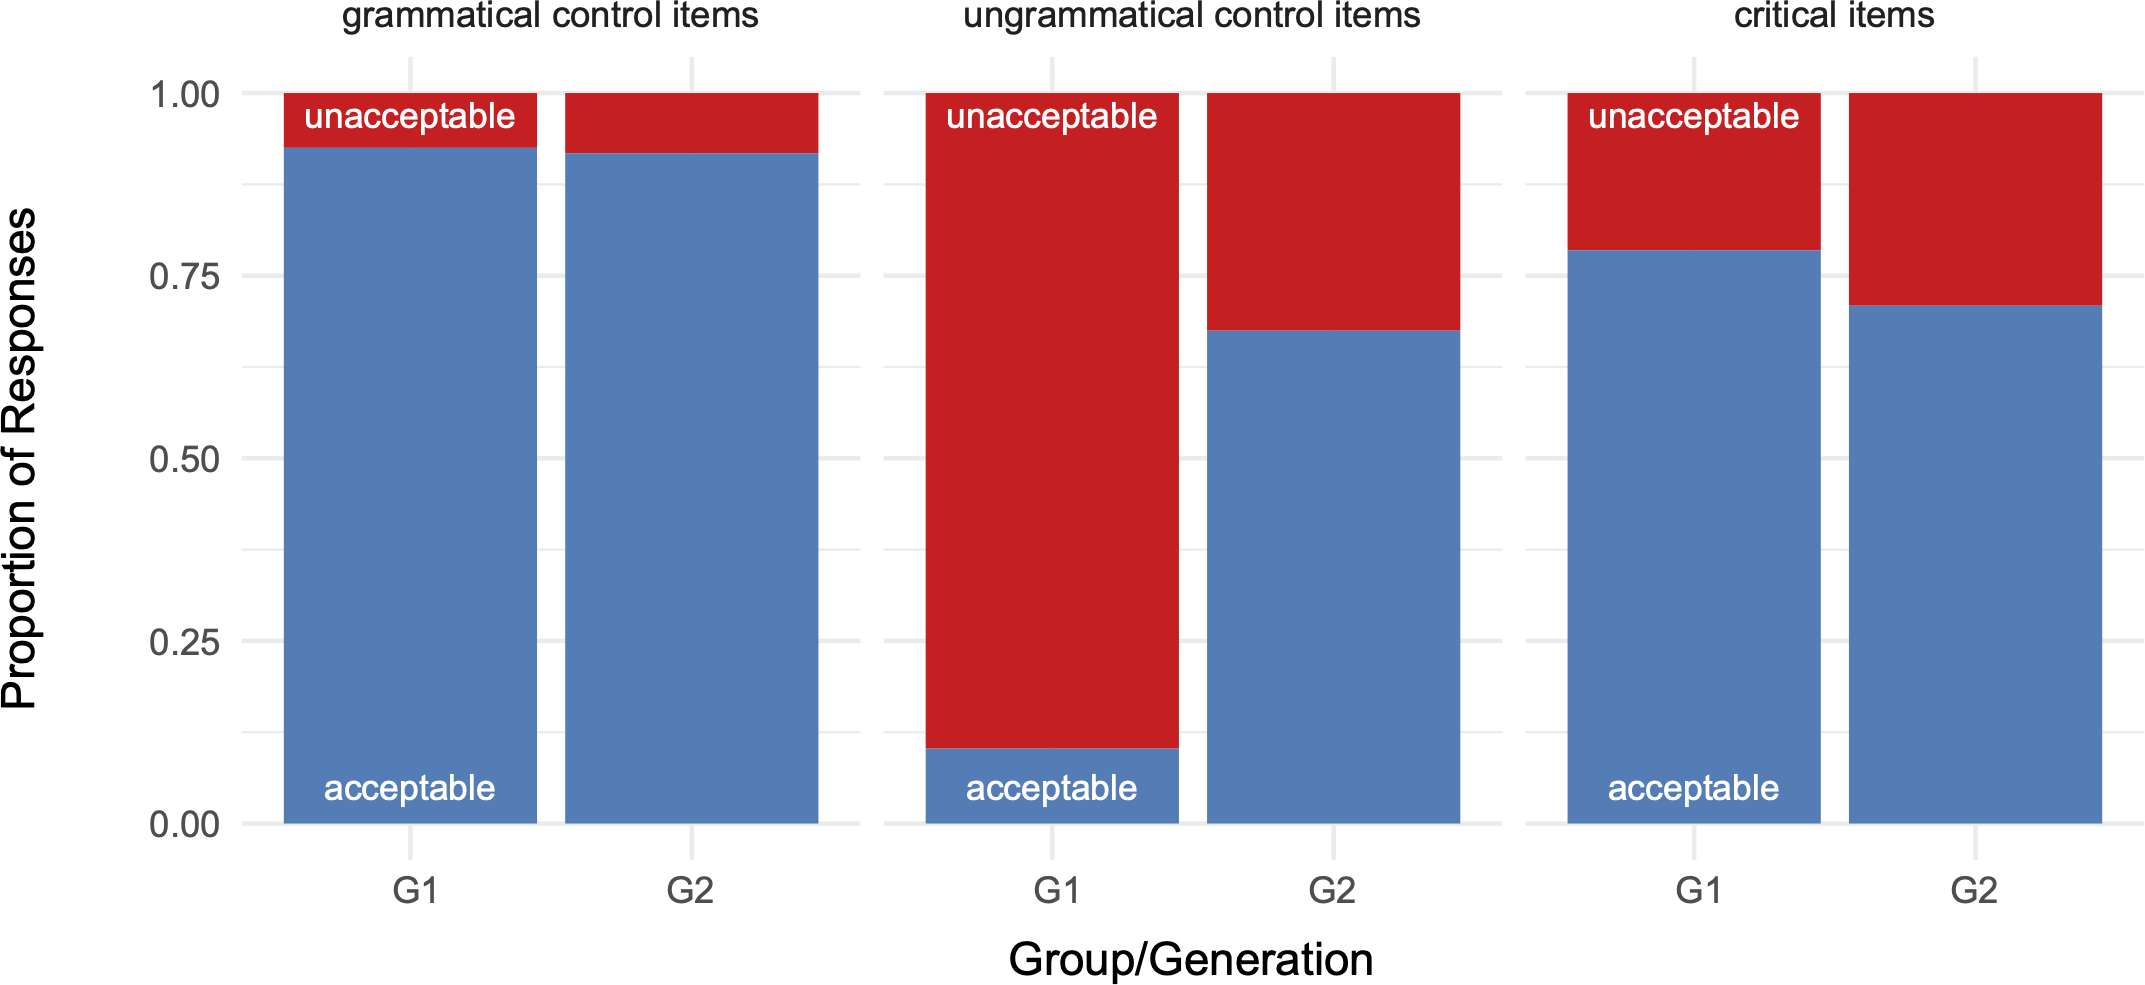
\includegraphics[width=\textwidth]{figures/Fig1.png}
\caption{Distribution of responses in the acceptability judgement task by item type (grammatical control, ungrammatical control, critical) and group (G1, G2). Blue and red indicate, respectively, responses accepting and responses rejecting the test items.}
\label{fig:AJT}
\end{figure}

Starting with the first comparison, as shown in \figref{fig:AJT}, both G1 and G2 were more likely to accept than reject grammatical control items; however, the similarity between G1 and G2 on grammatical control items was not seen in ungrammatical control items, which G2 was much more likely to accept than G1 was (consistent with the “yes-bias” documented for HSs; \citealt{Polinsky2018}). The group disparity in accepting ungrammatical control items specifically was reflected in an analysis of variance (ANOVA) on Model 1 using the \texttt{Anova()} function in the \texttt{car} package \citep{FoxWeisberg2019}. The ANOVA revealed no main effect of Group [$\chi^{2}(1)=0.783,\allowbreak p=0.376$] but a significant main effect of ItemType [$\chi^{2}(1)=19.648,\allowbreak p<0.001$] and a significant Group $\times$ ItemType interaction [$\chi^{2}(1)=27.428,\allowbreak p<0.001$]. 


\begin{table}
\caption{Fixed effects in Model 1 of the likelihood of accepting test items (grammatical control, ungrammatical control, critical) in the acceptability judgement task [$N=484$, log-likelihood $=-221.1$]. Intercept represents Group = G1, ItemType = grammatical control. Significance code: *** $p<0.001$.}
\label{tab:modelAJT}
\begin{tabular}{lrrrr@{\,}l}
\lsptoprule
Predictor & \multicolumn{1}{c}{$\beta$} & \multicolumn{1}{c}{SE} & \multicolumn{1}{c}{$z$} & \multicolumn{1}{c}{$\text{Pr}(>|z|)$} & \\
\midrule
(Intercept)                                & $2.947 $ & 0.786 & $3.748 $ & $<0.001$ & $^{***}$ \\
Group: G2                                  & $-0.003$ & 0.887 & $-0.003$ & 0.997 & \\    
ItemType: ungrammatical                    & $-5.483$ & 0.962 & $-5.699$ & $<0.001$ & $^{***}$ \\
ItemType: critical                         & $-1.334$ & 0.755 & $-1.768$ & 0.077 & \\  
Group: G2 $\times$ ItemType: & \\
\quad ungrammatical & $3.540 $ & 1.013 & $3.493 $ & $<0.001$ & $^{***}$ \\
\quad critical      & $-0.477$ & 0.830 & $-0.575$ & 0.566 & \\  
\lspbottomrule
\end{tabular}
\end{table}

The fixed-effects coefficients of Model 1 are summarized in \tabref{tab:modelAJT}. The results of Model 1 indicated that G1 was significantly more likely to accept grammatical control items compared to the null hypothesis, i.e. 50--50 odds [$\beta=2.947,\allowbreak p<0.001$]; crucially, however, G1 was also significantly less likely to accept ungrammatical than grammatical control items [$\beta=-5.483,\allowbreak p<0.001$]. G2 did not significantly differ from G1 in terms of likelihood of accepting grammatical control items [$\beta=-0.003,\allowbreak p=0.997$]. However, for G2, the reduction in likelihood of accepting ungrammatical control items compared to grammatical ones was significantly smaller than seen in G1 [$\beta=3.540,\allowbreak p<0.001$], suggesting that G2 did not reject ungrammatical control items as readily as G1 did.


Turning to the second comparison, as shown in \figref{fig:AJT}, both G1 and G2 were more likely to accept than reject critical items, much like grammatical control items. However, in general, participants were less likely to accept critical items than grammatical control items. Crucially, the results of Model 1 indicated little difference between G1 and G2 in this respect. G1 was not significantly more or less likely to accept critical items compared to grammatical control items [$\beta=-1.334,\allowbreak p=0.077$]. Furthermore, the \texttt{Group:G2 $\times$ ItemType:critical} interaction coefficient was negative but not significant [$\beta=-0.477,\allowbreak p=0.566$], meaning that the reduction in likelihood of accepting critical items compared to grammatical control items was statistically similar for G2 relative to G1. In short, the general similarity between G2 and G1 on grammatical control items was also reflected in the critical items containing the Twi diminutive suffix (crucially, the same items elicited in the picture description task), meaning that any between-group disparity in use of the morphological strategy is unlikely to be due to group differences in the suffix's acceptability per se.


\subsection{Morphological parsing results}
\label{MPTResultsSec}

Responses in the Twi morphological parsing task were analyzed to calculate a Twi morphological awareness score for each participant. Participants received a point for every target morpheme boundary they identified, and these points were then totaled. Participants' raw point totals were then converted to $z$-scores by group. For G2, who also completed an English morphological parsing task, we used the same method to calculate individual English morphological awareness scores; however, ultimately only the Twi morphological awareness scores were used as a predictor in the model of the picture description results. Although raw Twi morphological awareness scores were, on average, slightly higher for G1 ($M=23.4, SD=4.3$) than G2 ($M=19.9, SD=4.0$), this difference was not significant [Welch-corrected two-sample $t(12.5)=1.967, p=0.072$].

To get a picture of whether participants analyzed the Twi diminutive suffix as a separate morpheme, we also calculated the percentage of target diminutive morpheme boundaries identified by each group. This analysis showed that the majority of diminutive morpheme boundaries were successfully identified by G1 ($M=79.1\%, SD=23.1$) and by G2 ($M=71.3\%, SD=18.4$), suggesting that both groups represented the Twi diminutive suffix as a distinct unit in the Twi grammar (and not as merely lexicalized in the words in which the suffix occurs). Thus, this result supports interpreting any disproportionate use of the syntactic strategy for expressing diminutive meaning in Twi by G2 as representing an innovative preference rather than the loss of the diminutive morpheme (see research question 2 in \sectref{QuestionsHypothesisSec}).

\subsection{Verbal fluency results}
\label{VFTResultsSec}

Raw scores in the verbal fluency task were tabulated as the number of items named by participants for a target domain. Because each participant was assigned two domains, the second of which varied across participants, the raw scores from the two options for the second domain (habitat, animals) were compared statistically to check for a domain effect on naming performance. This comparison showed that, although scores tended to be higher on the “animals” domain ($M=8.6, SD=6.1$) than the “habitat” domain ($M=6.8, SD=2.4$), the difference between these domains was not significant [Welch-corrected two-sample $t(15.5)=1.009, p=0.328$]. Consequently, for the purposes of generating by-participant verbal fluency scores to use as a predictor in the model of the picture description results, we calculated a composite score for each participant by summing the number of unique items named across both domains. As expected, the raw composite scores were significantly higher for G1 than G2 [G1: $M=28.9, SD=7.2$; G2: $M=17.8, SD=5.5$; $t(10.6)=3.885, p=0.003$]. The raw composite scores were subsequently converted to $z$-scores by group, and the standardized scores were used in modeling.

\subsection{Picture description results}
\label{PDTResultsSec}

To examine participants' likelihood of using the morphological strategy for talking about smallness, responses in the picture description task were coded in binary fashion as either “morphological” or “non-morphological”. Responses in the “morphological” category included responses with the diminutive suffix only (e.g. \textit{sekam-ma} `knife'), responses where an adjectival construction was produced initially and then a suffixed form was produced (e.g. \textit{sekan ketewa} `knife' and then \textit{sekam-ma} `knife'), and responses where a simplex form was produced initially and then a suffixed form was produced (e.g. \textit{sekan} `machete' and then \textit{sekam-ma} `knife'). Responses in the “non-morphological” category included responses with an adjectival construction only, responses with a simplex form only, and responses where a simplex form was produced initially and then an adjectival construction was produced. Responses that included a diminutive suffix and an adjective within the same form ($N=4$, all produced by G1; 1\% of all responses) were considered ambiguous in terms of preference for the morphological strategy and were therefore excluded from analysis. 


The distribution of responses across categories is shown in \figref{fig:PDT}, which separates “syntactic + morphological” responses (i.e. those where an adjectival construction was produced before the final suffixed form was produced) and excludes the very few combined suffix-with-adjective responses for clarity. As shown in \figref{fig:PDT}, G1 and G2 differed markedly from each other in terms of preferences for expressing diminutive meaning, G1 preferring the morphological strategy and G2 the syntactic strategy. To analyze participants' response data statistically, we built two additional mixed-effects logistic regression models on the likelihood of producing the morphological diminutive (Models 2 and 3). Model 2 focused on the aforementioned group difference (see research question 1 in \sectref{QuestionsHypothesisSec}) and contained the fixed effect \textsc{Group} (treatment-coded; reference level = G1). Model 3 focused on the efficacy of individual-difference variables for predicting individual variation, particularly in G2 (research question 3); thus, Model 3 contained fixed effects for Twi morphological awareness score (\textsc{MorphAwareness}) and Twi verbal fluency score (\textsc{Fluency}), both standardized by group. Both models had a random-effects structure consisting of random intercepts by \textsc{Participant} and by \textsc{Item}.\largerpage

\begin{figure}
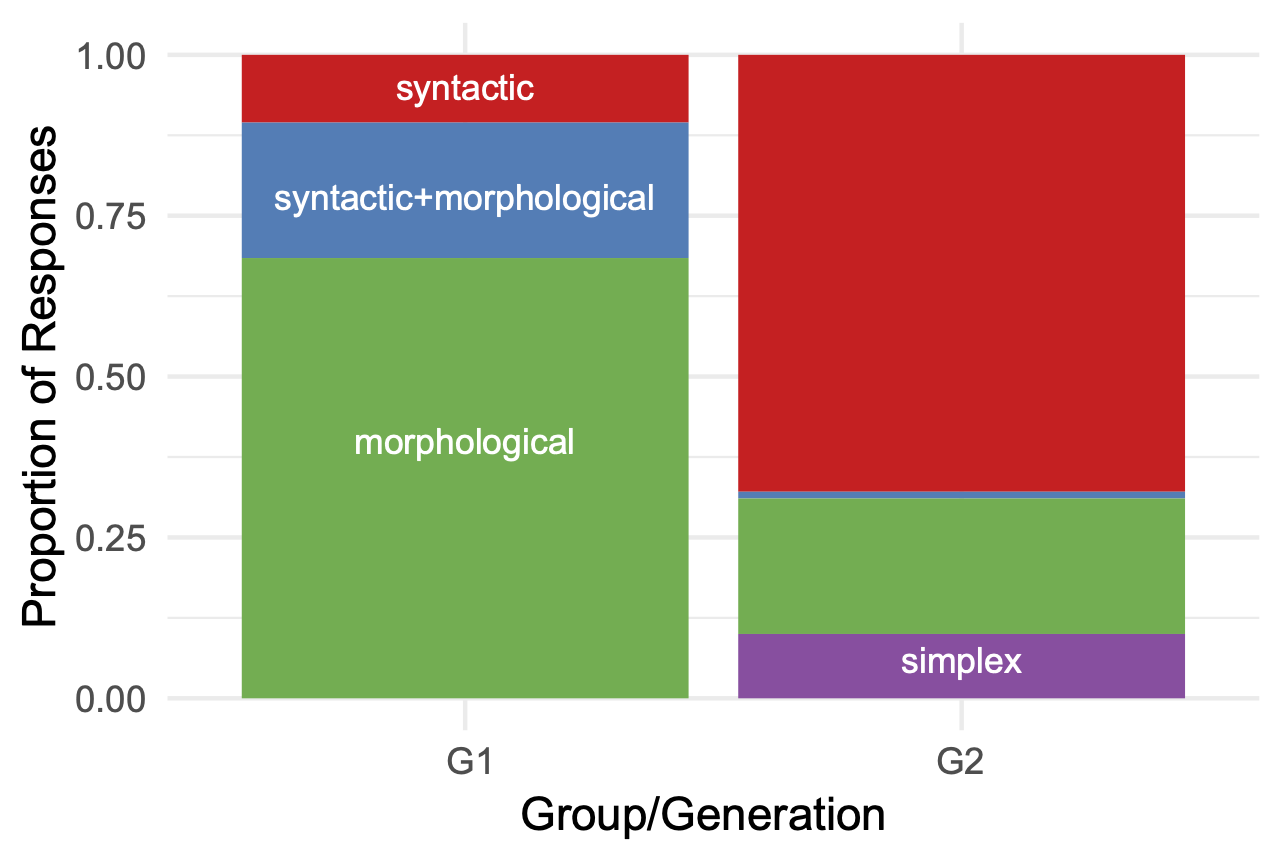
\includegraphics[width=.75\textwidth]{figures/Fig2.png}
\caption{Distribution of responses in the picture description task by group (G1, G2). The two main categories of response are “morphological” (i.e. diminutive suffix) and “non-morphological” (e.g. syntactic: adjectival construction). Responses marked as “syntactic\,+\,morphological” (initial use of an adjectival construction, final use of a diminutive suffix) were grouped into the “morphological” category for analysis. Responses marked as “simplex” (no diminutive) were grouped into the “non-morphological” category for analysis.}
\label{fig:PDT}
\end{figure}

Results of Model 2 confirmed that the group difference evident in \figref{fig:PDT} was statistically significant. In particular, G2 was much less likely to produce the morphological diminutive than G1 [$\beta=-6.366, z=-5.869, p<0.001$].{\interfootnotelinepenalty=10000\footnote{As mentioned in \sectref{ProcedureSec}, the experimenter sometimes switched into English to facilitate the testing procedure with G2. To explore whether such language switches may have affected G2's behavior, we conducted a post hoc analysis by pseudo-randomly selecting half of the critical trials including all G2 participants, transcribing the speech produced in these trials, and counting the number of instances of the experimenter switching into English. This analysis revealed that, in this set of 100 trials, the experimenter switched to English 19\% of the time. However, rates of morphological strategy use were identical between trials with and trials without a switch (switch: 4/19 = 21\%; no-switch: 17/81 = 21\%), suggesting that the experimenter's switching into English did not play a significant role in G2's observed strategy use.}}

Turning to Model 3, we found evidence of an effect of verbal fluency but not of morphological awareness. The fixed-effect coefficients of Model 3 (summarized in \tabref{tab:modelPDT}) indicated that, at average levels of \textsc{MorphAwareness} and \textsc{Fluency} (i.e. $z$-score of zero), the odds of G2 producing the morphological diminutive were significantly lower than 50–50 [$\beta=-1.987, p=0.035$]. At average levels of \textsc{Fluency}, higher levels of \textsc{MorphAwareness} were not associated with a significantly higher likelihood of producing the morphological diminutive [$\beta=0.020, p=0.941$]. On the other hand, at average levels of \textsc{MorphAwareness}, higher levels of \textsc{Fluency} were associated with a significantly higher likelihood of producing the morphological diminutive [$\beta=0.992, p=0.026$], and the interaction coefficient did not indicate a significant change in this effect at higher levels of \textsc{MorphAwareness} [$\beta=-0.746, p=0.068$]. 

\begin{table}
\caption{Fixed effects in Model 3 of the likelihood of G2 producing a morphological diminutive in the picture description task [$N=190$, log-likelihood $=-64.2$]. Significance code: * $p<0.05$.}
\label{tab:modelPDT}
\begin{tabular}{lrrrc@{\,}l}
\lsptoprule
Predictor & \multicolumn{1}{c}{$\beta$} & \multicolumn{1}{c}{SE} & \multicolumn{1}{c}{$z$} & \multicolumn{1}{c}{$\text{Pr}(>|z|)$} & \\
\midrule
(Intercept)                     & $-1.987$  & 0.941 & $-2.111$ & 0.035 & $^{*}$ \\ 
MorphAwareness                  & $0.020 $  & 0.276 & $0.074 $ & 0.941 & \\
Fluency                         & $0.992 $  & 0.445 & $2.227 $ & 0.026 & $^{*}$ \\
MorphAwareness $\times$ Fluency & $-0.746$  & 0.409 & $-1.822$ & 0.068 & \\
\lspbottomrule
\end{tabular}

\end{table}

As a final part of the analysis of individual-difference variables, we inspected the omnibus correlation of each of \textsc{MorphAwareness} and \textsc{Fluency} with individual G2 participants' overall rate (proportion) of morphological diminutive production. As shown in \figref{fig:IDscatterplots} (and consistent with \figref{fig:PDT} showing the group pattern), at an individual level, G2 did not show particularly high rates of morphological diminutive production; crucially, however, these rates were almost all higher than zero, meaning that few G2 participants showed evidence of loss of the diminutive suffix. As for \textsc{MorphAwareness} and \textsc{Fluency}, the correlation analyses showed that these variables were not significantly correlated with each other for G2 [Pearson's $R=0.383, t(17)=1.707, p=0.106$]. Furthermore, morphological diminutive production was not significantly correlated with \textsc{MorphAwareness} [Pearson's $R=0.263, t(17)=1.122, p=0.277$], but was significantly, and moderately, correlated with \textsc{Fluency} [Pearson's $R=0.476, t(17)=2.233, p=0.039$].

\begin{figure}
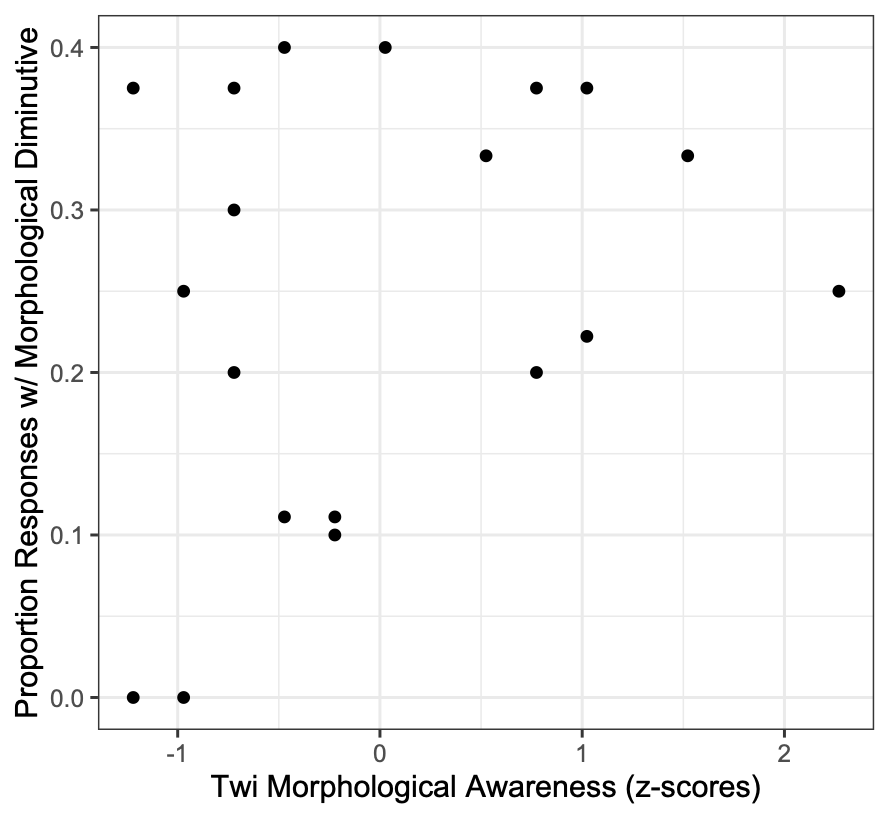
\includegraphics[width=0.5\textwidth]{figures/Fig3a.png}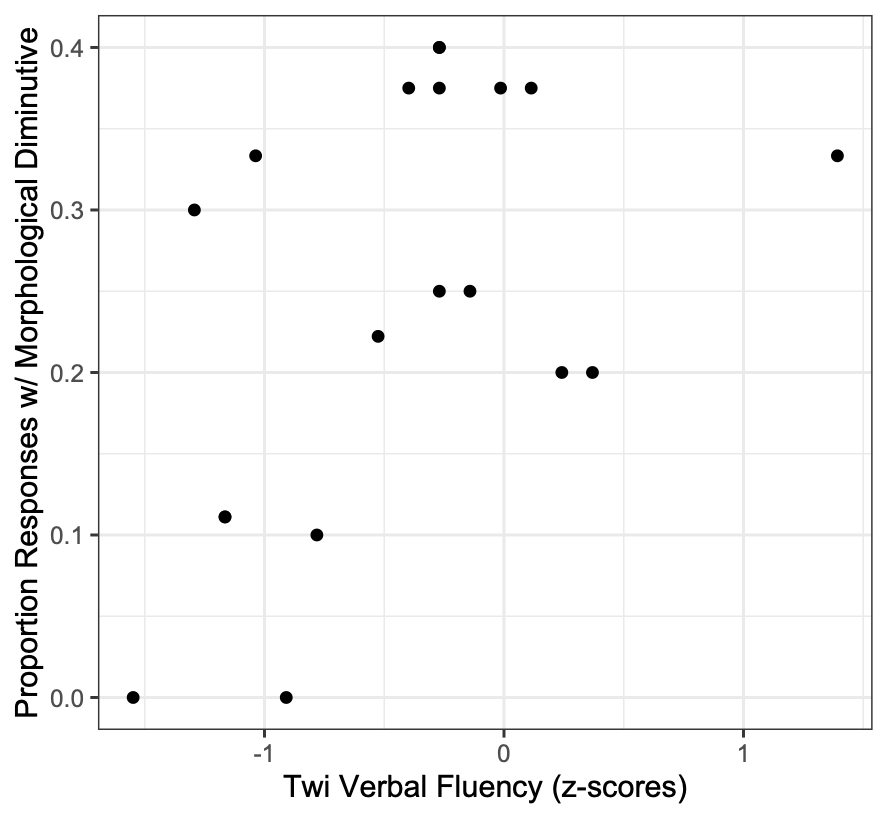
\includegraphics[width=0.5\textwidth]{figures/Fig3b.png}
\caption{Scatterplots of G2's proportions of morphological diminutive production by Twi morphological awareness score (left) and verbal fluency score (right). Each dot represents one G2 participant.}
\label{fig:IDscatterplots}
\end{figure}

Taken together, the results of Model 3 and the correlation analyses point to verbal fluency as a stronger predictor of G2's morphological diminutive production than morphological awareness. However, we regard this finding with caution, as we observed rather high levels of morphological awareness among the G2 participants in this study overall (see \sectref{MPTResultsSec}). Thus, it is possible that the predictive power of morphological awareness in Twi may differ with a G2 sample evincing a wider range of morphological awareness.

\section{Discussion}
\label{DiscussionSec}

Returning to our hypotheses outlined in \sectref{QuestionsHypothesisSec}, recall that the current study tested three hypotheses (H1--H3) about English-dominant, second-generation (G2) Twi speakers' knowledge of the diminutive suffix (i.e. the morphological diminutive) and their relative preferences for the morphological and syntactic strategies of expressing diminutive meaning in Twi. Combining results from four tasks (acceptability judgment, morphological parsing, verbal fluency, and picture description), the findings of this study generally provided support for H1--H3. We consider each hypothesis in turn below.

First, we hypothesized that, whereas first-generation (G1) Twi speakers would show a preference for the morphological strategy of expressing diminutive meaning, G2 would show a preference for the syntactic strategy (H1). Results of the picture description task were consistent with H1: G1 strongly preferred the morphological strategy, using the diminutive suffix well over half of the time, but G2 consistently preferred the syntactic strategy, using the diminutive suffix less than half of the time at both the group level and the individual level (see \figref{fig:IDscatterplots}). Thus, English-dominant G2 Twi speakers in the US do indeed show a different pattern with respect to strategies for expressing the semantic notion of smallness as compared to adult G1 speakers. Because the morphological strategy is incrementally more complex than the syntactic strategy (i.e. relative to the complexity that G2 must master for basic use of the HL apart from the diminutive), this finding is superficially consistent with the tendency of HSs to simplify complex linguistic phenomena in the HL. 

Crucially, however, G2's bias toward the syntactic strategy does not reflect their having failed to acquire the morphological diminutive. On the contrary, despite the complexities associated with the morphological diminutive, the vast majority of G2 participants produced the morphological diminutive at least part of the time they needed to express diminutive meaning in the picture description task, suggesting they have not simplified the HL grammar by eliminating the morphological strategy entirely. This finding thus supports our hypothesis that G2's preference for the syntactic strategy, while stronger than G1's, is not categorical (H2). Results from the acceptability judgment and morphological parsing tasks further suggest that G2 generally represents the morphological diminutive in the HL grammar. First, G2 did not perform significantly differently from G1 on critical items with the diminutive in the acceptability judgement task. Second, G2 parsed the diminutive suffix as a meaningful unit in the Twi morphological parsing task. These results are inconsistent with a scenario in which G2 speakers have not acquired the morphological diminutive.

Turning to variation in G2, we found partial support for our hypothesis that individual differences in Twi morphological awareness and Twi verbal fluency would predict variation in G2's rates of morphological diminutive use (H3). In particular, we found an effect of verbal fluency, but not of morphological awareness: G2 participants with higher verbal fluency scores were more likely to produce a morphological diminutive in the picture description task. However, we also observed that G2's morphological awareness scores in Twi were high overall -- in fact, not significantly different from G1's -- leaving open the possibility of observing an effect of morphological awareness with a wider range in morphological awareness. Thus, further study of the role of morphological awareness in morphological diminutive use would be a useful direction for future research.

In connection with G2's observed preference for the syntactic strategy, it is important to note that virtually all of the G2 participants in this study had indeed acquired the post-nominal adjective syntax associated with the syntactic strategy. Because adjective order is thought to be an early-acquired aspect of core syntax \citep[mastered as early as age 2; see][]{Brown1973, ParadisNicoladisGenesee2000, Nicoladis2002} and is consistently post-nominal throughout the Twi language (i.e., not just for the purposes of expressing the diminutive), we expected G2 to successfully manage the inhibitory complexity of using the syntactic strategy with target-like post-nominal adjective order (and not to transfer the competing pre-nominal adjective order of English), even if their preference for the syntactic strategy itself might be English-influenced. In accordance with this expectation, almost all the G2 participants consistently produced the post-nominal adjective order in Twi; further, of the two G2 participants who did not, only one showed clear evidence of transferring the English order to Twi, producing the English order in nearly all target items. Crucially, the overwhelmingly target-like production of Twi adjective order is inconsistent with the idea of unconstrained dominant language transfer to the weaker language, as has been suggested in other bilingual studies \citep[e.g.,][]{YipMatthews2000}. Under the assumption that adjective order is part of core syntax, this finding instead supports the idea that early-acquired, core areas of the grammar in the weaker language remain stable over time and resistant to CLI \citep{SoraceFiliaci2006, Sorace2011}, although there may be the occasional exceptional case as we observed in this study.\largerpage[-1]

We are still left to explain what exactly is responsible for the observed divergence in linguistic preferences between G2 and G1, and we end this section by discussing the possible contributions of complexity, CLI, and universal tendencies. To begin, we believe that complexity -- in particular, minimization of complexity -- plays a role. As discussed in \sectref{QuestionsHypothesisSec}, for a variety of reasons, the morphological strategy of expressing diminutive meaning in Twi can be considered incrementally more complex than the syntactic strategy for English-dominant speakers (i.e. G2). Consequently, the finding of a strong preference in G2 for the syntactic strategy -- or, to put it another way, G2's move away from the morphological strategy preferred by G1 -- is consistent with a tendency for HSs to minimize the complexity of using their HL. The operative word here is ``minimize'', as opposed to ``eliminate'' or ``simplify'' complexity, however, because it bears repeating that G2 still uses the morphological strategy, just less often than G1 does; that is, complexity minimization underlies the preferences, but not the availability of the strategies themselves. Converging evidence of complexity minimization comes from other aspects of G2's responses in the picture description task as well. For example, whereas G1 consistently distinguished \textit{sekamma} `knife' (a diminutivized form) and \textit{sekan} `machete' (a simplex form), and \textit{adɔmma} `little bell' (diminutivized) and \textit{ɛdɔn} `bell' (simplex), some G2 participants did not do so consistently, producing simplex forms in critical trials that called for the diminutive (see \figref{fig:PDT}). This type of response minimizes complexity by conflating lexical distinctions and avoiding phonological rules that apply with the diminutive, although it does not necessarily indicate that the speaker would never make these distinctions or apply these rules.

CLI can also account for the divergent preferences of G2 vis-{\`a}-vis G1, and we believe that it plays a role as well. Because the syntactic strategy is preferred in the dominant language, English, G2's preference for the syntactic strategy in Twi can be interpreted as reflecting CLI from English preferences (or, to put it another way, from the relative strength of the syntactic strategy in English, where it is generally preferred over the morphological strategy). But, as above, if G2's preference for the syntactic strategy can be explained in terms of complexity minimization, why posit that CLI is involved at all? There is one aspect of our results that points to this conclusion. As mentioned above, we found that there were two G2 participants who, unlike other G2 participants, used pre-nominal adjective order to implement the syntactic strategy at least part of the time. Because this pre-nominal adjective order is ostensibly due to CLI from English, CLI must be invoked to explain these participants' production. Therefore, seeing no reason to believe that CLI is limited to adjective order, we assume that CLI also plays a role in the use of the syntactic strategy itself; it is just that, for most G2 speakers, this CLI is not allowed to extend into the core syntax of the HL.\largerpage[-2]

As for universal tendencies, we do not consider it likely that a universal tendency is responsible for G2's preference for the syntactic strategy, because there is no clear typological or developmental evidence for a universal tendency that would favor the syntactic strategy. In regard to typology, we expect such a tendency to be reflected in a bias toward analytic languages (e.g. diachronic changes resulting in synthetic languages becoming more analytic, but not the other way around). Further, in first language development, such a tendency should produce a bias toward analytical constructions (e.g. two-word phrases emerging before bimorphemic words). To our knowledge, however, neither of these hypothetical biases is strongly supported in the literature; this includes the recent literature on creoles, which suggests that ``creoles are not more analytic than the other [lexifier] varieties'' \citep[49]{SiegelSzmrecsanyiKortmann2014}. Thus, we conclude that G2's preference for the syntactic strategy is not due to a universal tendency, but instead attributable to complexity minimization and CLI.

\section{Conclusion}
\label{ConclusionSec}

In closing, we would like to acknowledge two limitations of this study, which point out directions for future research on the web of factors involved in shaping HSs' linguistic preferences in their HL. First, our sample of G2 Twi speakers (HSs) was relatively small and possibly showed unusually high morphological awareness. Second, the task we used to measure diminutive production ultimately focused on elicited speech, which may not reflect how HSs express diminutive meaning in naturalistic speech communication. Thus, it would be useful in future work to replicate and extend the current findings with a larger, socio-demographically more diverse participant sample and with a task paradigm that more closely mimics spontaneous conversational speech.

Finally, another direction for future research is to begin to tease apart the effects of complexity and CLI, which are confounded in the current findings. In our case of Twi-English bilingualism, complexity minimization and CLI from English both favor the syntactic strategy of expressing diminutive meaning, so it is impossible to know for sure what the relative contribution of each factor is to G2's observed preference for the syntactic strategy. This type of question could be addressed by examining other cases of preferences in HS bilingualism, where complexity minimization favors one option but CLI from the dominant majority language favors a different option. Research in this vein would improve our understanding of the unique role of complexity in influencing HSs' use of their HL.


\section*{Acknowledgments}
The authors gratefully acknowledge funding from the Department of Linguistics at Boston University, support from the Seventh-Day Adventist Church in Massachusetts and New York in reaching the Twi community, and helpful feedback from anonymous reviewers and audience members at the Bilingualism, Mind, and Brain Lab meeting and the 47th Boston University Conference on Language Development (BUCLD 47). 

\printbibliography[heading=subbibliography,notkeyword=this]
\end{document}
